\documentclass{article}

\usepackage{amssymb, amsmath, amsthm, verbatim, graphicx}

\begin{document}

\large

\begin{center}
\textbf{Homework  12} \\  
\end{center}

\normalsize

Reading
\begin{itemize}
\item Section $8.3$ covers undirected graphical models.
\item Section $1.2.3$ provides a general discussion of Bayesian probability.  Bishop uses Bayesian models throughout the text, we have just not emphasized them previously.
\end{itemize}

\begin{enumerate}
% fall 2019, hw 12
\item The file \verb+HW12_problem1.txt+ contains $50$ iid samples, $\hat{X}_1, \hat{X}_2,\dots, \hat{X}_{50}$, from a one-dimensional random variable $X$..  Assume that $X \sim \mathcal{N}(\mu, \sigma^2)$ where $\sigma^2$ is known with $\sigma^2 = 1$.  Our goal is to estimate $\mu$.   Let $\bar{x}$ be the sample mean and $N=50$.
\begin{enumerate}
\item Show that the maximum likelihood estimate (MLE) of $\mu$ is given by the sample mean $\bar{x}$.
\item Taking a Bayesian approach, assume a normal prior on $\mu$, $\mu \sim \mathcal{N}(0, \beta^2)$ with $\beta = 10$.  Let $f(\mu)$ be the pdf of the prior.  Let $p(\mu)$ be the posterior.   Show,
\begin{equation}
p(\mu) = \frac{1}{Z} P(\hat{X}_1, \hat{X}_2,\dots, \hat{X}_{50} \  | \ \mu) f(\mu),
\end{equation}
where
\begin{equation}
Z = \int_{-\infty}^\infty P(\hat{X}_1, \hat{X}_2,\dots, \hat{X}_{50} \ | \ \mu) f(\mu) d\mu.
\end{equation}
Then show
\begin{equation}
p(\mu) \sim \mathcal{N}(\frac{\bar{x}}{1 + \frac{\sigma^2}{\beta^2N}}, \frac{\sigma^2 \beta^2}{N\beta^2 + \sigma^2})
\end{equation}
Graph $p(\mu)$ using the data.
Hint:  use completing the squares to combine a product of exponentials into a single exponential.
(Here you're showing that for random mean and fixed variance, the normal distribution is a conjugate prior to itself)
\item Again take a Bayesian approach, but this time assume a prior $f(\mu)$,
\begin{equation}
f(\mu) = \bigg\{
\begin{array}{cc}
\frac{1}{10} & \text{if } x \in [5,7] \\
4 & \text{if } x \in [9,9.2] \\
0 & \text{otherwise}
\end{array}
\end{equation}
In this case the posterior $p(\mu)$ is not normally distributed.  Graph $p(\mu)$ and compare to the graph in (b).   (Hint:  you can compute $Z$ using a numerical integration function.  In R, \textbf{integrate}).
\end{enumerate}

% fall 2019, hw 12
%\item The attached file \verb+HW12_problem2.txt+ contains $200$ rows.  The ith row contains a $y_i, x^{(i)}_1, x^{(i)}_2$ values.   Assume the linear model $y_i \sim a_0 + a_1x^{(i)}_1 + a_2x^{(i)}_2 + \epsilon_i$ where the $\epsilon_i$ are iid draws from  $\mathcal{N}(0, \sigma^2)$,   Our goal is to infer $a_0, a_1, a_2, \sigma^2$.  
%\begin{enumerate}
%\item Write down an equation for the MLE  of $a_0, a_1, a_2, \sigma^2$ and compute the estimates given the data.  (Hint:  you can derive a matrix equation, i.e. the normal equations, for the values of the $a_i$).
%\item Take a Bayesian approach.  Assume any prior you like on the parameters.   Write down an expression for the posterior $p(a_0, a_1, a_2, \sigma^2)$.   Generate $4$ histograms, a histogram for the distribution of each of the four parameters, respectively.     To generate the histograms, run a Metropolis-Hastings MCMC that samples from the posterior. 
%\item Compare (a) and (b)
%\end{enumerate} 

% fall 2018, hw 8
\item This problem relates to the figure below, which is Figure $17.3$ in the book Elements of Statistical Learning.   Let $W$ be a $3$-dimensional r.v.  Typically we write $W = (W_1, W_2, W_3)$, but to match the figure, let $W = (X, Y, Z)$.   Suppose that $X, Y, Z$ are each in $\{-1, 1\}$.   Consider three parametrizations of a probabilities distrubution for $W$, i.e. a joint probability distribution for $X, Y, Z$.   Let $\eta = (\eta_1, \eta_2, \eta_3)$.
\begin{align} \label{1}
P(X=x, Y=y, Z=z) & =\alpha \exp[\eta_1x + \eta_2y + \eta_3z - w_{12} xy - w_{13} xz] \\
\label{2}
P(X=x, Y=y, Z=z) & =\alpha \exp[\eta_1x + \eta_2y + \eta_3z - w_{12} xy - w_{13} xz - w_{23} yz] \\ 
\label{3}
P(X=x, Y=y, Z=z) & = \alpha \exp[\eta_1x + \eta_2y + \eta_3z - w_{12} xy - w_{13} xz - w_{23} yz - w_{123} xyz],
\end{align}
where the $\alpha$ is a normalizing constant that differs between the three distributions. (In the lecture I used $1/Z$ for the normalization, but here $Z$ is one of the random variables.)
\begin{enumerate}
\item Show that for distribution (\ref{1}), $Y \perp Z | X$ so that the edge between $Y$ and $Z$ in the graph is not consistent with the distribution.  Show that for distribution (\ref{1}), we can write
\begin{equation}
P(X=x, Y=y, Z=z) = \alpha \psi_1(x,y) \psi_2(x,z)
\end{equation}
corresponding to the maximal clique form of the Hammersley-Clifford Theorem.  What are the cliques in this case?
\item Show that for distributions (\ref{2}) and (\ref{3}), no pair of the three r.v. $X, Y, Z$ is conditionally independent given the third r.v., making each edge in the graph necessary for consistency with the probability distribution.  (Note: this reflects the comment  directly below the figure: \textit{A graphical model does not always uniquely specify the higher-order structure of a joint probability distribution}.)  
\item Consider distribution (\ref{1}).  Let $\eta_i = 1/2$ for $i=1,2,3$.  Let $w_{12} = 1$, $w_{13} = -1$.  Use a Monte-Carlo approach based on a Metropolis-Hastings sampler to estimate the correlation between $X$ and $Y$.  (Since the graph is so small, in this case we could directly compute the correlation by summing through all possible values of $W$, but this would not be the case if the dimension of $W$ was, say, $20$.)
\end{enumerate}


\begin{figure}[h]
%\centering
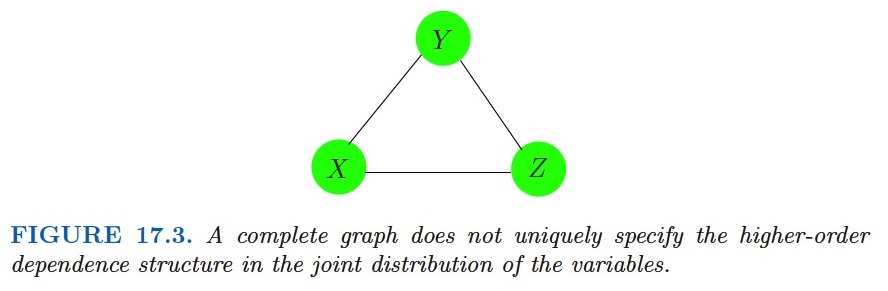
\includegraphics[width=.95\textwidth]{ESM_Fig_17_3.jpg}
\end{figure}



\end{enumerate}


\end{document}
